%-----------------------------------------------------------------------------
%
%               Template for sigplanconf LaTeX Class
%
% Name:         sigplanconf-template.tex
%
% Purpose:      A template for sigplanconf.cls, which is a LaTeX 2e class
%               file for SIGPLAN conference proceedings.
%
% Guide:        Refer to "Author's Guide to the ACM SIGPLAN Class,"
%               sigplanconf-guide.pdf
%
% Author:       Paul C. Anagnostopoulos
%               Windfall Software
%               978 371-2316
%               paul@windfall.com
%
% Created:      15 February 2005
%
%-----------------------------------------------------------------------------


\documentclass[preprint]{sigplanconf}

% The following \documentclass options may be useful:

% preprint      Remove this option only once the paper is in final form.
% 10pt          To set in 10-point type instead of 9-point.
% 11pt          To set in 11-point type instead of 9-point.
% authoryear    To obtain author/year citation style instead of numeric.

\usepackage{amsmath}
%\usepackage{silence}
\usepackage{pgf}
\usepackage{tikz}
\usetikzlibrary{arrows,automata}
\usepackage{url}
\usepackage[hidelinks]{hyperref}
\usepackage{fancyvrb}
\usepackage[numbers]{natbib}
%\WarningsOff

\begin{document}
\fvset{fontsize=\small}
\newcommand{\idris}{\textsc{Idris}}
\newcommand{\idata}{\textsf{iData}}
\newcommand{\itasks}{\textsf{iTasks}}
\special{papersize=8.5in,11in}
\setlength{\pdfpageheight}{\paperheight}
\setlength{\pdfpagewidth}{\paperwidth}

\conferenceinfo{IFL '13}{August 28--31, 2013, Nijmegen, The Netherlands} 
\copyrightyear{2013} 
\copyrightdata{978-1-nnnn-nnnn-n/yy/mm} 
\doi{nnnnnnn.nnnnnnn}

% Uncomment one of the following two, if you are not going for the 
% traditional copyright transfer agreement.

%\exclusivelicense                % ACM gets exclusive license to publish, 
                                  % you retain copyright

%\permissiontopublish             % ACM gets nonexclusive license to publish
                                  % (paid open-access papers, 
                                  % short abstracts)

\titlebanner{}        % These are ignored unless
\preprintfooter{}   % 'preprint' option specified.

\title{Practical Dependently-Typed Programming for the Web}
\subtitle{Correct and Secure Web Programming using Dependent Types and Embedded Domain-Specific Languages}
%\subtitle{Using Embedded Domain-Specific Languages to Improve Confidence in Web Applications}

\authorinfo{Simon Fowler \and Edwin Brady}
           {School of Computer Science, University of St Andrews, St Andrews, Scotland}
           {Email: \{sf37, ecb10\}@st-andrews.ac.uk}

\maketitle

\begin{abstract}
Dependently-typed languages allow very expressive types to be used during development, in turn facilitating easier reasoning about the operation of programs written in such languages. Stronger type specifications do however bring with them the disadvantage
that it becomes increasingly difficult to write programs that are accepted by
the type checker and additional proofs may have to be specified by a user.

Embedded domain-specific languages (EDSLs) address this problem by introducing
a layer of abstraction over more specific underlying types, allowing
domain-specific code to be written in high-level languages which use dependent
types to enforce certain invariants without additional proof obligations. 

In this paper, we apply this technique to web programming, and introduce an
EDSL to facilitate the creation and handling of web forms which retain type
information, reducing the scope for programmer error and attacks such as SQL
injection. We also show how to enforce resource usage
protocols associated with common web operations such as CGI, database access
and session handling.  

\end{abstract}

%\category{CR-number}{subcategory}{third-level}

% general terms are not compulsory anymore, 
% you may leave them out
%\terms
%term1, term2

%\keywords
%keyword1, keyword2

\section{Introduction}

Web applications, whilst ubiquitous, are also prone to incorrect construction
and security exploits such as SQL injection \cite{owasp:sqli} or cross-site
scripting \cite{owasp:xss}. Security breaches using such exploits are
far-reaching, and high profile cases involve large corporations such as Sony,
who suffered a well-publicised and extremely costly SQL Injection breach in
2011 \cite{ieee:sony}, and \textit{Yahoo!}, who suffered a breach in 2012
\cite{imperva:yahoo}. 

Many web applications are written in dynamically-checked scripting languages
such as PHP, Ruby or Python, which facilitate rapid development
\cite{w3techs:webpls}. A significant drawback, however, is that such languages
do not provide  the same static guarantees about runtime behaviour afforded by
programs with more expressive, static type systems, instead relying on
extensive unit testing to ensure correctness and security. 

%%------- EXAMPLE
Let us consider a simple database access routine, written in
PHP, where we wish to obtain the name and address of every employee working in
a given department, \texttt{\$dept}. We firstly construct an object
representing a database connection, where the arguments are the database host,
user, password and name respectively:


%
\begin{Verbatim}
  $conn = new mysqli("localhost", "username", 
                     "password", "db");
\end{Verbatim}
%
We then check to see if the connection was successful, and exit
if not.  This check is optional, so
it would be possible to omit it. However, this would cause
problems with later steps.

%
\begin{Verbatim}
  if (mysqli_connect_errno()) {
      exit();
  }
\end{Verbatim}
%
We then create a prepared statement detailing our query, and bind the
\texttt{`dept'} value:

\begin{Verbatim}
  $stmt = $conn->prepare("SELECT `name`, `address` 
     FROM `staff` WHERE `dept` = ?);
  $stmt->bind_param('s', $dept);
\end{Verbatim}
%
After the parameters have been bound, we execute the statement, assign
variables into which results will be stored, and fetch each row in turn. 
Failure to execute a statement before attempting to fetch rows would cause an error, as would attempting to execute a statement without binding variables to it.

%
\begin{Verbatim}
  $stmt->execute();
  $stmt->bind_result($name, $address);
  while ($stmt->fetch()) {
    printf("Name: %s, Age: %s", $name, $age);
  }
\end{Verbatim}
%
Finally, once the statement and connection are no longer needed, they should be
closed in order to discard the associated resources:

%
\begin{Verbatim}
  $stmt->close();
  $conn->close();
\end{Verbatim}
%
Even in this small example, there exists a specific resource usage protocol.
Firstly, a connection to the database must be opened. The object-oriented style
used in the example encapsulates this to an extent, as the object must be
created in order for operations to be performed, however it is less obvious in
a procedural version of the code. Secondly, a prepared statement is created,
using the raw SQL and placeholders to which variables are later bound. The
statement is then executed, and each row is retrieved from the database.
Finally, the resources are freed. 

Problems may arise if the protocol is not followed correctly.
A developer may, for example, accidentally close a statement whilst still
retrieving rows, which would cause a runtime error. Similarly, a programmer may
omit closing the statement or connection, which can lead to
problems such as resource leaks in longer-running server applications.
However, in conventional programming languages, there is no way to check
automatically that a protocol is followed.

In contrast, the use of \textit{dependent types} makes it possible
to specify a program's behaviour precisely, and to check that a 
specification is followed.
%
The difficulty is 
that automatic verification by a compiler can be difficult or
often impossible, requiring additional proofs to be given by the programmer.

This complexity can be ameliorated through the use of \textit{embedded
domain-specific languages} (EDSLs), which aim to abstract away the
complexity of the underlying type system. EDSLs allow domain experts to
write verified domain-specific code, with the EDSL itself providing the implicit proof that the written code is correct.

\idris{} \cite{brady2011idris} is a language with full dependent types, and
extensive support for EDSLs through overloading and syntax macros. Through the
use of \idris{}, and a framework for describing resource protocols using
\emph{algebraic effects}~\cite{brady:effects}, we
present a dependently-typed web framework, which allows the construction of
programs with additional guarantees about correctness and security, whilst
minimising the increase in development complexity. 

\subsection{Contributions}
The primary contribution of this paper is the application of 
dependent types to provide strong static guarantees
about the correctness and security of web applications, whilst minimising
additional development complexity. In particular, we present:

\begin{itemize}
\item A form-handling mechanism, which preserves type information and
manages user input, therefore
increasing applications' resilience to attacks such as SQL injection and cross-site scripting.

\item Representations of CGI, Databases and sessions as
\textit{resource-dependent algebraic effects}, allowing programs to be accepted only when they
follow clearly defined resource usage protocols.

\item A message board application, demonstrating the usage of the framework.

\end{itemize}

We structure the remainder of this paper as follows. We provide a brief
overview of the \texttt{Effects} framework in Section ~\ref{effects}; explain
how this may be used to ensure adherence to resource usage protocols for CGI,
SQLite and a session handler in Section ~\ref{rup}; describe an EDSL for
type-safe form handling in Section ~\ref{form}, implemented using
\texttt{Effects}; and discuss the larger example
of a message board system making use of these components in Section
~\ref{messageboard}.

The code used to implement the framework and all associated examples used in this paper is available online at \url{http://www.github.com/SimonJF/IdrisWeb}.
% =================================================
% =================================================

\section{An overview of the \texttt{Effects} framework}
\label{effects}

\texttt{Effects}~\cite{brady:effects} is an \idris{} library which handles
side-effects such as state, exceptions, and I/O as \emph{algebraic
effects}~\cite{Plotkin2009}. In particular, it supports parameterising effects
by an input and output \emph{state}, which permits effectful programs to track
the progress of a resource usage protocol. Effectful programs are written
in a monadic style, with \texttt{do}-notation, with their type stating which
specific effects are available.
Effectful
programs are described using the following data type,
in the simplest case:

\begin{Verbatim}
Eff : (m : Type -> Type) ->
      (es : List EFFECT) -> (a : Type) -> Type
\end{Verbatim}

\texttt{Eff} is parameterised over a \emph{computation context}, \texttt{m}, 
which describes the context in which the effectful program will be run, a
list of side effects \texttt{es} that the program is permitted to use, and the
program�s return type \texttt{a}. The name \texttt{m} for the computation context is
suggestive of a monad, but there is no requirement for it to be so.

For example, the following type carries an integer state,
throws an exception of type \texttt{String} if the state reaches 100, 
and runs in a \texttt{Maybe} context:

\begin{Verbatim}
addState : Eff Maybe [STATE Int, EXCEPTION String] ()
addState = do val <- get
              when (val == 100) (raise "State too big")
              put (val + 1)
\end{Verbatim}

\subsection{Implementing Effects}

Effects such as state and exception are described as algebraic data types,
and run by giving \emph{handlers} for specific computation contexts. 
Effects have a corresponding \emph{resource} (in the case of state, the
resource is simply the current state). Executing an effectful operation may
change the resource and return a value:

\begin{Verbatim}
Effect : Type
Effect = (in_res : Type) -> (out_res : Type) -> 
         (val : Type) -> Type
\end{Verbatim}

For example, the state effect is described as follows:

\begin{Verbatim}
data State : Effect where
     Get :      State a a a
     Put : b -> State a b ()
\end{Verbatim}

That is, \texttt{Get} returns a value of type \texttt{a} without updating
the resource type. \texttt{Put} returns nothing, but has the effect of updating
the resource. In order to make an effect usable, we implement a handler
for a computation context by making an instance of the following class:

\begin{Verbatim}
class Handler (e : Effect) (m : Type -> Type) where
     handle : res -> 
              (eff : e res res' t) -> 
              (k: res' -> t -> m a) -> m a
\end{Verbatim}

The \texttt{handle} function takes the input resource, an effect which may
update that resource and execute a side-effect, and a continuation \texttt{k}
which takes the updated resource and the return value of the effect. We use
a continuation here primarily because there is no restriction on the number of
times a handler may invoke the continuation (raising an exception, for example,
will not call the continuation). Reading and updating states in handled
for all computation contexts \texttt{m} as follows:

\begin{Verbatim}
instance Handler State m where
     handle st Get     k = k st st
     handle st (Put n) k = k n ()
\end{Verbatim}

Finally, we promote \texttt{State} into a concrete effect \texttt{STATE}, and
the \texttt{Get} and \texttt{Put} operations into functions in \texttt{Eff}, as
follows:

\begin{Verbatim}
STATE : Type -> EFFECT
STATE t = MkEff t State

get : Eff m [STATE x] x
get = Get 

put : x -> Eff m [STATE x] ()
put val = Put val
\end{Verbatim}

A concrete effect is simply an algebraic effect type paired with its current
resource type. This, and other
technical details, are explained in full elsewhere~\cite{brady:effects}.
For the purposes of this paper, it suffices to know how to describe and
handle new algebraic effects.

\subsection{Resource Protocols as Effects}

More generally, a program might modify the set of effects available.
This might be desirable for several reasons, such as adding a new
effect, or to update an index of a dependently typed state. In this
case, we describe programs using the \texttt{EffM} data type:

\begin{Verbatim}
EffM : (m : Type -> Type) ->
       (es : List EFFECT) -> (es' : List EFFECT) ->
       (a : Type) -> Type
\end{Verbatim}

\texttt{EffM} is parameterised over the context and type as before, but
separates input effects (\texttt{es}) from output effects (\texttt{es'}). 
In fact, \texttt{Eff}
is defined in terms of \texttt{EffM}, with equal input/output effects.
We can use this to describe how effects follow resource protocols. A simple
example is a file access protocol, where a file must be opened before it
is read or written, and a file must be closed on exit:

\begin{Verbatim}
data FileIO : Effect where
     Open  : String -> (m : Mode) -> 
             FileIO () (OpenFile m) ()
     Close : FileIO (OpenFile m) () ()

     ReadLine  : FileIO (OpenFile Read)  
                        (OpenFile Read) String
     WriteLine : String -> 
                 FileIO (OpenFile Write) 
                        (OpenFile Write) ()
     EOF       : FileIO (OpenFile Read)  
                        (OpenFile Read) Bool
\end{Verbatim}

Note that the types of the input and output resources describes how resource
state changes in each operation: opening a file changes an empty resource to
a resource containing an open file; reading a line is only possible if the
resoource is a file open for reading, etc.
The handler for this effect for an \texttt{IO} computation context will
execute the required primitive I/O actions, as well as throwing an exception
if any operation fails.

The following program type checks, and therefore implicitly carries 
a proof that the file resource protocol is followed correctly:

\begin{Verbatim}
testFile : Eff IO [FILE_IO (), STDIO] () 
testFile = catch (do open "testFile" Read
                     str <- readLine
                     close
                     putStrLn str)
                 (\err => putStrLn ("Error: " ++ show err))
\end{Verbatim}


The type of \texttt{testFile} states
that File I/O and console I/O are available effects, and in particular that
the resource associated with the File I/O will be in the same state on entry
and exit.
Therefore, attempting to write to the file, or failing to open or close the
file, would cause a \emph{compile-time} error. 

We will use this technique extensively
throughout this paper: describe a resource usage protocol in terms of
state transitions; implement an effect which captures that protocol; implement
programs which, by using this effect, implicitly carry a proof that the resource
protocol has been correctly followed.


% =================================================
% =================================================

\section{Modelling resource usage protocols}
\label{rup}
In this section, we show how three such effects; CGI, database access and a simple session handler, may be implemented, and describe the benefits of developing programs using this technique over simply handling them in the IO context or as part of a monad transformer.

% =================================================

\subsection{CGI}
%TODO: Fix up the labels
\begin{figure}[htpb!]
\centering
\scalebox{0.8}{
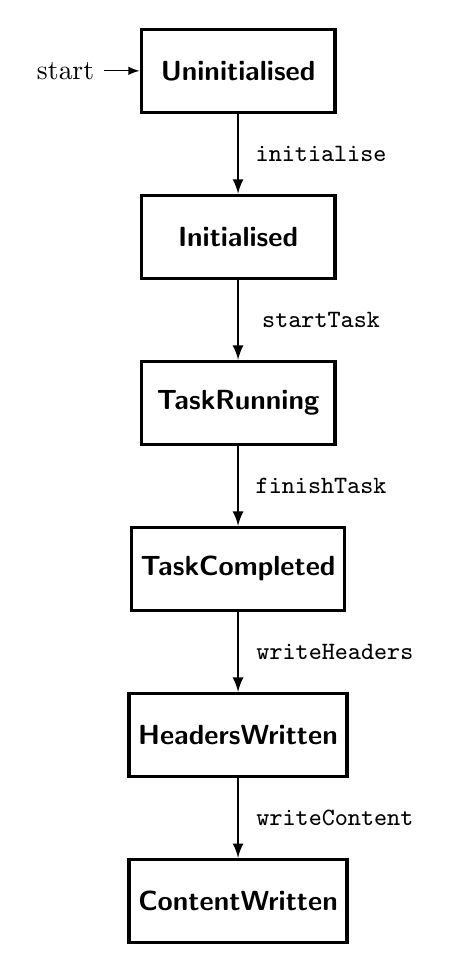
\begin{tikzpicture}[>=latex]
  \tikzstyle{state} = [draw, very thick, fill=white, rectangle, minimum height=3em, minimum width=7em, node distance=6em, font={\sffamily\bfseries}]
  
  \tikzstyle{stateEdgePortion} = [black,thick];
  \tikzstyle{stateEdge} = [stateEdgePortion,->];
  \tikzstyle{edgeLabel} = [pos=0.5, font={\sffamily\small}];

  \node[initial,state] (A)              {Uninitialised};
  \node[state]         (B) [below of=A] {Initialised};
  \node[state]         (C) [below of=B] {TaskRunning};
  \node[state]         (D) [below of=C] {TaskCompleted};
  \node[state]         (E) [below of=D] {HeadersWritten};
  \node[state]         (F) [below of=E] {ContentWritten};

  \path (A) edge[stateEdge]   node[edgeLabel, xshift=3em] {\texttt{initialise}} (B)
        (B) edge[stateEdge]   node[edgeLabel, xshift=3em] {\texttt{startTask}} (C)
        (C) edge[stateEdge]   node[edgeLabel, xshift=3em] {\texttt{finishTask}} (D)
        (D) edge[stateEdge]   node[edgeLabel, xshift=3.5em] {\texttt{writeHeaders}} (E)
        (E) edge[stateEdge]   node[edgeLabel, xshift=3.5em] {\texttt{writeContent}} (F);
\end{tikzpicture}
}
\caption{CGI States}
\label{fig:cgistates}
\end{figure}

CGI is used to invoke an application on a web server, making use of environment variables to convey information gained from an HTTP request and using standard output to communicate with the remote client. Importantly, HTTP headers must be correctly written to the browser prior to any other output; failure to do so will result in an internal server error being shown.

A previous implementation of CGI in \idris{} implemented CGI an extension of monadic IO, as in Haskell. Whilst basic functionality worked correctly, this approach had several disadvantages; most notably, it was possible to perform arbitrary IO at any point in the program. If this were to happen, then the program would fail due to the fact that headers had not been written to the client.

By modelling CGI as a resource-dependent algebraic effect, we may enforce a resource usage protocol which, even though the program may be running in an IO execution context, prevents arbitrary IO from being performed and therefore ensures that the headers are written correctly. In order to accomplish this, we define an effect, \texttt{Cgi}, and an associated resource, \texttt{InitialisedCGI}, which is parameterised over the current state, \texttt{CGIStep}. This resource describes the current state, alongside a \texttt{CGIInfo} record which contains information from the request. We represent an uninitialised CGI process as the unit type, ().
\begin{Verbatim}[samepage]
data CGIStep = Initialised 
             | TaskRunning 
             | TaskCompleted 
             | HeadersWritten 
             | ContentWritten

data InitialisedCGI : CGIStep -> Type where
  ICgi : CGIInfo -> InitialisedCGI s
\end{Verbatim}
Figure~\ref{fig:cgistates} shows the states through which the CGI program
progresses, and Figure~\ref{fig:cgieffect} shows how this is represented
as a resource-dependent algebraic effect. Each operation performed in an effectful
program requires the resource to be of a certain type, and the completion of
the operation may alter the type or value of the resource.

Upon creation, the CGI application is uninitialised, meaning that environment variables have not been queried to populate the CGI state. The only operation
that can be performed in this state is initialisation: by calling
\texttt{initialise}, a CGIInfo record is populated, and the state transitions
to \texttt{Initialised}. The \texttt{Init} operation is defined as part of the
\texttt{Cgi} effect, and involves transitioning from the uninitialised state to
the initialised state.

\begin{figure}[h]
\begin{Verbatim}
data Cgi : Effect where
    Init : Cgi () (InitialisedCGI Initialised) ()
    StartRun : Cgi (InitialisedCGI Initialised) 
                   (InitialisedCGI TaskRunning) ()
    FinishRun : Cgi (InitialisedCGI TaskRunning) 
                    (InitialisedCGI TaskCompleted) ()
    WriteHeaders : Cgi (InitialisedCGI TaskCompleted) 
                       (InitialisedCGI HeadersWritten) ()
    WriteContent : Cgi (InitialisedCGI HeadersWritten) 
                       (InitialisedCGI ContentWritten) ()
    OutputData : String -> 
                 Cgi (InitialisedCGI TaskRunning) 
                     (InitialisedCGI TaskRunning) ()
    RunAction : Env IO (CGI (InitialisedCGI TaskRunning) 
                               :: effs) -> 
                       CGIProg effs a -> 
                       Cgi (InitialisedCGI TaskRunning) 
                           (InitialisedCGI TaskRunning) a
\end{Verbatim}
\caption{CGI Effect}
\label{fig:cgieffect}
\end{figure}

Additional operations, including those to query POST and GET variables, are omitted in the interest of brevity.

User code executes in the \texttt{TaskRunning} state. Several operations, such as querying the POST and GET variables, are available in this state, alongside functions to output data to the web page and append data to the response headers. It is important to note, that at this stage nothing is written to the page, with the \texttt{output} and \texttt{addHeader} functions instead modifying the CGIInfo record. This data may then be printed at the end of the program's execution, in accordance with the resource usage protocol.

After the user code has finished execution, control returns to the library code. At this point, the state transitions to TaskCompleted, and the headers are written.
Finally, the headers and content are written which completes the process. Since we parameterise the resource over a state, we may ensure that certain operations only happen in a particular prescribed order.

In \idris{}, types are first-class, meaning that they may be treated like other terms in computations. We may therefore define the following type synonym, which we may use in order to make use of the CGI framework: 
\begin{Verbatim}
CGIProg : List EFFECT -> Type -> Type
CGIProg effs a = 
 Eff IO (CGI (InitialisedCGI TaskRunning) :: effs) a
\end{Verbatim}
This is then passed, along with initial values for other effects that the user may wish to use, to the runAction function, which invokes the RunAction operation and executes the user-specified action.

A simple ``Hello, world!'' program would be defined as follows:

\begin{Verbatim}
module Main
import Cgi

sayHello : CGIProg [] ()
sayHello = output "Hello, world!"

main : IO ()
main = runCGI [initCGIState] sayHello
\end{Verbatim}
% =================================================

\subsection{Database access with SQLite}

%TODO: Fix up the labels
\begin{figure}[htpb!]
\centering
\scalebox{0.8}{
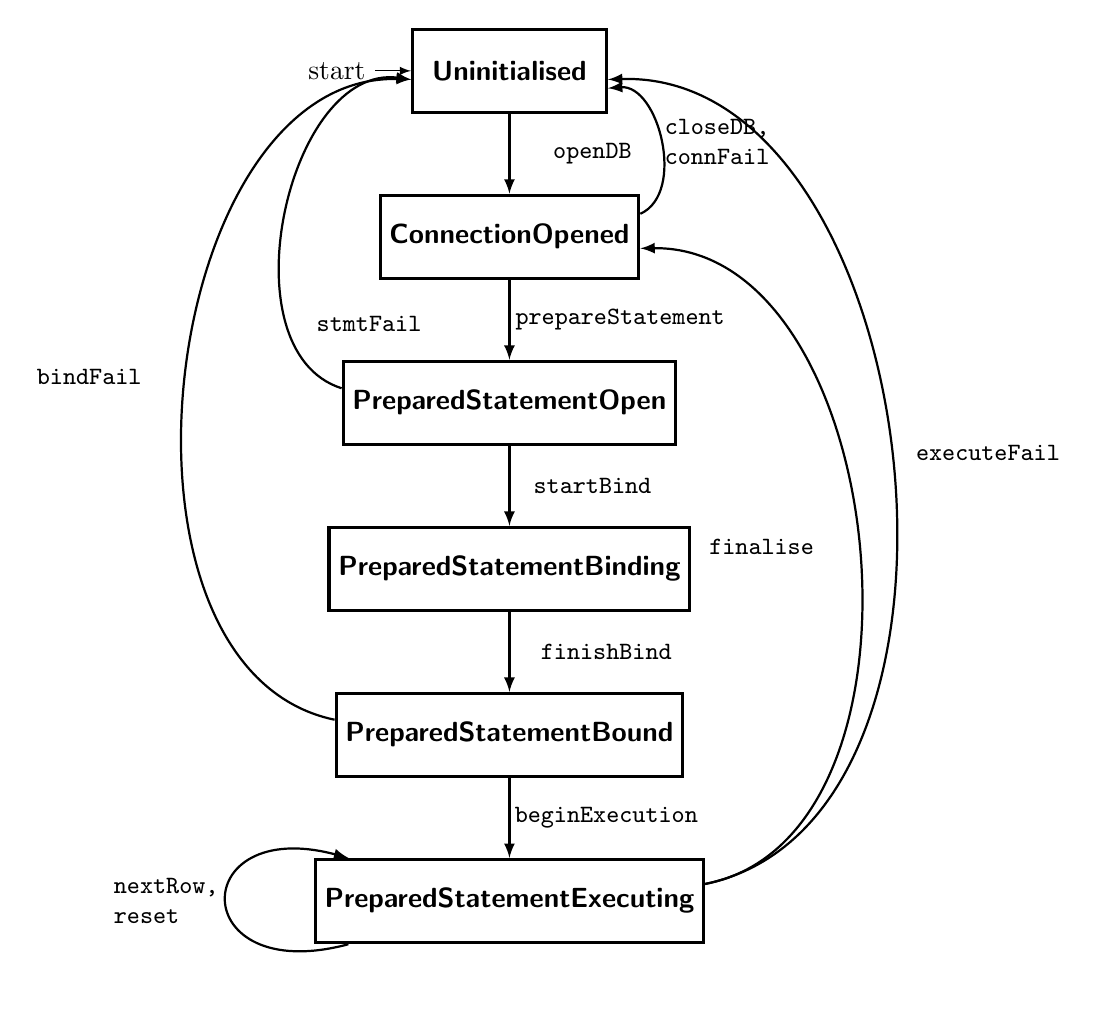
\begin{tikzpicture}[>=latex]
  \tikzset{every loop/.style={min distance=10mm,looseness=5}}
  \tikzstyle{state} = [draw, very thick, fill=white, rectangle, minimum height=3em, minimum width=7em, node distance=6em, font={\sffamily\bfseries}]
  
  \tikzstyle{stateEdgePortion} = [black,thick];
  \tikzstyle{stateEdge} = [stateEdgePortion,->];
  \tikzstyle{edgeLabel} = [pos=0.5, font={\sffamily\small}];

  \node[initial,state] (A)              {Uninitialised};
  \node[state]         (B) [below of=A] {ConnectionOpened};
  \node[state]         (C) [below of=B] {PreparedStatementOpen};
  \node[state]         (D) [below of=C] {PreparedStatementBinding};
  \node[state]         (E) [below of=D] {PreparedStatementBound};
  \node[state]         (F) [below of=E] {PreparedStatementExecuting};

  \path (A) edge[stateEdge]   node[edgeLabel, xshift=3em] {\texttt{openDB}} (B)
        (B) edge[stateEdge, bend right=80]   node[edgeLabel, text width=2cm, xshift=3em] {\texttt{closeDB, connFail}} (A)
        (B) edge[stateEdge]   node[edgeLabel, xshift=4em] {\texttt{prepareStatement}} (C)
        (C) edge[stateEdge, bend left=85]   node[edgeLabel, xshift=3em, yshift=-4em] {\texttt{stmtFail}} (A)
        (C) edge[stateEdge]   node[edgeLabel, xshift=3em] {\texttt{startBind}} (D)
        (D) edge[stateEdge]   node[edgeLabel, xshift=3.5em] {\texttt{finishBind}} (E)
        (E) edge[stateEdge, bend left=85]   node[edgeLabel, xshift=-3.5em] {\texttt{bindFail}} (A)
        (E) edge[stateEdge]   node[edgeLabel, xshift=3.5em] {\texttt{beginExecution}} (F)
        (F) edge[stateEdge, bend right=85]   node[edgeLabel, xshift=-3.5em] {\texttt{finalise}} (B)
        (F) edge[stateEdge, bend right=85]   node[edgeLabel, xshift=3.5em] {\texttt{executeFail}} (A)
            edge[stateEdge, loop left]   node[edgeLabel, text width=2cm, xshift=2em] {\texttt{nextRow, reset}} (B);
\end{tikzpicture}
}
\caption{Database Resource Usage Protocol}
\label{fig:sqlitestates}
\end{figure}


SQLite\footnote{\texttt{http://www.sqlite.org}} is a lightweight SQL database engine often used as simple, structured storage for larger applications. We make use of SQLite due to its simplicity, although we envisage that these concepts would be applicable to more complex database management systems. 

The creation, preparation and execution of SQL queries has a specific usage protocol, with several possible points of failure. Failure is handled in traditional web applications by the generation of exceptions, which may be handled in the program.
Handling such exceptions is often optional, however, and in some cases unhandled errors may cause a deployed web application to display an error to the user. Such errors can be used to determine the structure of an insecure SQL query, and are often used by attackers to determine attack vectors for SQL injection attacks.

Figure~\ref{fig:sqlitestates} shows a resource usage protocol for database
access, which we have implemented for the SQLite library. This is encapsulated
by the \texttt{Sqlite} effect (Figure \ref{fig:dbeffect}; we again omit some operations, such as those to
bind and retrieve data types other than \texttt{String}, in the interest of
brevity).

\begin{figure}[h]
\begin{Verbatim}[samepage]
data Sqlite : Effect where
  OpenDB : 
    String -> 
    Sqlite () 
           (SQLiteRes ConnectionOpened) Bool
  CloseDB : 
    Sqlite (SQLiteRes ConnectionOpened) () Bool
  PrepareStatement : 
    String -> 
    Sqlite (SQLiteRes ConnectionOpened) 
           (SQLiteRes PreparedStatementOpen) Bool
  StartBind : 
    Sqlite (SQLiteRes PreparedStatementOpen) 
           (SQLiteRes PreparedStatementBinding) ()
  BindText : 
    ArgPos -> String -> Int -> 
    Sqlite (SQLiteRes PreparedStatementBinding) 
           (SQLiteRes PreparedStatementBinding) 
           Bool
  FinishBind : 
    Sqlite (SQLiteRes PreparedStatementBinding) 
           (SQLiteRes PreparedStatementBound) 
           Bool
  ExecuteStatement : 
    Sqlite (SQLiteRes PreparedStatementBound) 
           (SQLiteRes PreparedStatementExecuting) ()
  Finalise : 
    Sqlite (SQLiteRes PreparedStatementExecuting) 
           (SQLiteRes ConnectionOpened) 
           Bool
  GetColumnText : 
    Int -> 
    Sqlite (SQLiteRes PreparedStatementExecuting)
           (SQLiteRes PreparedStatementExecuting)
           String
  RowStep : 
    Sqlite (SQLiteRes PreparedStatementExecuting)
           (SQLiteRes PreparedStatementExecuting)
           StepResult
\end{Verbatim}
\caption{Database Effect}
\label{fig:dbeffect}
\end{figure}

There are three main phases involved in the usage of the SQLite protocol: connection to the database, preparation of a query, and execution of the query. This is reflected in the associated resource \texttt{SQLiteRes}, which again is parameterised by the current protocol state.
\begin{Verbatim}
data SQLiteRes : Step -> Type where
  OpenConn : DBPointer -> SQLiteRes s
  OpenStmt : DBPointer -> StmtPointer -> SQLiteRes s
  ExecutingStmt : DBPointer -> 
                  StmtPointer -> 
                  StepResult -> 
                  SQLiteRes s
                  
data DBPointer = ValidConn Ptr
               | InvalidConn

data StmtPointer = ValidStmt Ptr
                 | InvalidStmt 
\end{Verbatim}
If a failure happens at any point during the computation, the resource is updated to reflect the failure: if, for example, the library failed to create a connection to the database, the resource value would be updated to \texttt{OpenConn InvalidConn}. At this point, no further side-effecting requests are made to the underlying SQLite library, in order to ensure safety. The \texttt{connFail}, \texttt{stmtFail}, \texttt{bindFail} and \texttt{executeFail} utility functions allow for failures, once detected, to be handled by executing the appropriate sequence of state transition functions to dispose of any open resources and return to the initial protocol state. 

%Queries are evaluated through one or more calls to the \texttt{nextRow} function, which either executes an update statement or returns the next row of a result set. 
SQL queries are evaluated in SQLite upon a call to the C library function \texttt{sqlite3\_step()}. In the case that a statement returns a result set, each subsequent call retrieves another row for processing using a column access function. Once all rows have been retrieved, the library returns \texttt{SQLITE\_DONE}, meaning that no further calls should be made without resetting the function. We encapsulate this requirement through the \texttt{StepResult} data type within the \texttt{ExecutingStmt} constructor. 
\begin{Verbatim}
data StepResult = Unstarted
                | StepFail
                | StepComplete
                | NoMoreRows
\end{Verbatim}
Each call to \texttt{nextRow}, which is a wrapper around the underlying \texttt{sqlite3\_step()} C library function, returns a result of type \texttt{StepResult}, which is then reflected in the resource. Calls to \texttt{sqlite3\_step()} are only executed if the previous \texttt{StepResult} is either \texttt{Unstarted} or \texttt{StepComplete}. We may therefore statically guarantee that only calls that will return a valid result are executed. 

By incorporating pointers to open connections and prepared statements into the resource associated with the effect, we introduce a further layer of abstraction, in order to hide implementation details from the developer and encourage cleaner, less error-prone code. 

\subsubsection{Example Code}
Programs making use of the DSL should look familiar to developers even without a background in functional programming. To demonstrate the functionality of the library, we return to the previous example of selecting the names and addresses of all staff working in a given department. Due to the fact that the \texttt{Effects} library overloads the bind operator, we may make use of \texttt{do}-notation, facilitating the usage of an imperative style.

We define a function of type:
\begin{Verbatim}
String ->
Eff IO [SQLITE ()] (Either String (List (String, String)))
\end{Verbatim}
This means that the program will be run in the IO execution context, and must start and end with no active resources. The return type indicates that either a list of \text{(String, String)} pairs, representing names and addresses in the database, or an error will be returned. 
\begin{Verbatim}
testSelect : String -> Eff IO [SQLITE ()] 
             (Either String (List (String, Int)))
testSelect dept = do
  open_db <- openDB "people.db"
  if open_db then do
    let sql = "SELECT name, address FROM `staff` 
                    WHERE dept = ?;"
    sql_prep_res <- prepareStatement sql
    if sql_prep_res then do 
      startBind
      bindText 1 dept
      finishBind
      beginExecution
      results <- collectResults
      finaliseStatement
      closeDB
      return $ Right results
    else do err <- stmtFail
            return $ Left err
  else do err <- connFail
          return $ Left err 
\end{Verbatim}
The program initially attempts to open a connection to the \texttt{people.db} database. At this point, since the \texttt{OpenDB} operation has been invoked, the program transitions to the \texttt{ConnectionOpened} state. The \texttt{openDB} function returns a Boolean value indicating whether or not the operation is successful. If not, then the \texttt{connFail} function is called to generate an appropriate error and dispose of the resources, as shown in ~\ref{fig:sqlitestates}.

A call to \texttt{prepareStatement} attempts to create a prepared statement, and a subsequent call to \texttt{beginExecution} allows data to be retrieved from the database.

\texttt{CollectResults} is a simple function which makes a call to \texttt{nextRow} in order to make the next row of the result set available for processing, and uses the \texttt{getColumnText} and \texttt{getColumnInt} functions to retrieve the data from the database. This function is then recursively called until there are no more rows to process.
\begin{Verbatim}
collectResults : 
  Eff IO 
  [SQLITE (SQLiteRes PreparedStatementExecuting)] 
  (List (String, Int))
collectResults = do
  step_result <- nextRow
  case step_result of
      StepComplete => do name <- getColumnText 1
                         age <- getColumnInt 2
                         xs <- collectResults
                         return $ (name, age) :: xs
      NoMoreRows => return []
      StepFail => return [] 
\end{Verbatim}
In order to decrease unnecessary boilerplate code in user applications, we provide functions which abstract out unnecessary parts of this process. In order to do this, we define the algebraic data type \texttt{DBVal}, which is a tagged union over simple primitive types:
\begin{Verbatim}
data DBVal = DBInt Int
           | DBText String
           | DBFloat Float
           | DBNull
\end{Verbatim}
We also make use of the \texttt{ResultSet} type, which is a list of returned database rows.
\begin{Verbatim}
  ResultSet : Type
  ResultSet = List (List DBVal)
\end{Verbatim}
Using these, we may implement a function, \texttt{ExecuteSelect}, which, given a query, a list of variables to bind and their associated indices within the query, and a function which is used to extract information out of each returned database row, returns either a \texttt{ResultSet} or an error.
\begin{Verbatim}
executeSelect : 
  String -> String -> List (Int, DBVal) -> 
  (Eff m [SQLITE (SQLiteRes PreparedStatementExecuting)] 
                 (List DBVal)) -> 
  Eff m [SQLITE ()] (Either String ResultSet)
\end{Verbatim}
% =================================================
\subsection{A Simple Session Handler}
More complex web applications require some persistent state across separate requests. This is often done through an abstraction of a \textit{session}, wherein a cookie is set on the remote host containing a unique session ID, which is in turn used to retrieve data. In this section, we describe the implementation of a simple session handler, and the resource usage protocol involved. 

A major strength of the \texttt{Effects} library is that it allows for simple composition of individual, fine-grained effects. By combining the individual CGI and SQLite components, we may construct a simple session handler to provide a notion of state across separate web requests. 

We implement this by having a SQLite database, containing two tables: \texttt{session}, which stores session keys and their associated expiry dates, and \texttt{sessiondata}, which contains the data associated with each session. A datum associated with the session is described as a tagged union containing one of the primitive types \texttt{String}, \texttt{Bool} or \texttt{Int}, which is serialised alongside a type tag for storage in the database.
%TODO: Fix up the labels

\begin{figure}[h]
\begin{Verbatim}[samepage]
data Session : Effect where
  LoadSession : 
  SessionID -> 
  Session (SessionRes SessionUninitialised) 
          (SessionRes SessionInitialised) 
          (Maybe SessionData)
  UpdateSession : 
    SessionData -> 
    Session (SessionRes SessionInitialised) 
            (SessionRes SessionInitialised) ()
  CreateSession : 
    SessionData -> 
    Session (SessionRes SessionUninitialised) 
            (SessionRes SessionInitialised) 
            (Maybe SessionID)
  DeleteSession : 
    Session (SessionRes SessionInitialised) 
            (SessionRes SessionUninitialised) Bool 
  WriteToDB : 
    Session (SessionRes SessionInitialised) 
            (SessionRes SessionUninitialised) Bool
  DiscardSessionChanges : 
    Session (SessionRes SessionInitialised) 
            (SessionRes SessionUninitialised) ()
  GetSessionID : 
    Session (SessionRes SessionInitialised) 
            (SessionRes SessionInitialised) 
            (Maybe SessionID)
  GetSessionData : 
    Session (SessionRes SessionInitialised) 
            (SessionRes SessionInitialised) 
            (Maybe SessionData)
\end{Verbatim}
\caption{Session Effect}
\label{fig:sessioneffect}
\end{figure}

\begin{figure}[htpb!]
\centering
\scalebox{0.8}{
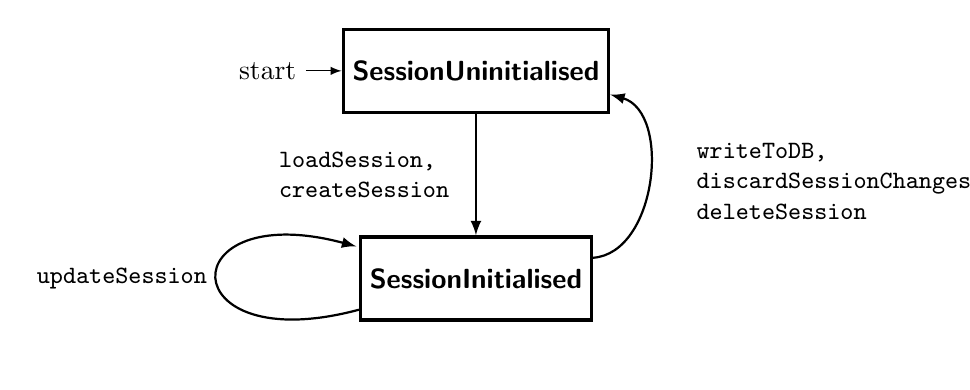
\begin{tikzpicture}[>=latex]
  \tikzstyle{state} = [draw, very thick, fill=white, rectangle, minimum height=3em, minimum width=7em, node distance=7.5em, font={\sffamily\bfseries}]
  
  \tikzstyle{stateEdgePortion} = [black,thick];
  \tikzstyle{stateEdge} = [stateEdgePortion,->];
  \tikzstyle{edgeLabel} = [pos=0.5, font={\sffamily\small}];

  \node[initial,state] (A)              {SessionUninitialised};
  \node[state]         (B) [below of=A] {SessionInitialised};

  \path (A) edge[stateEdge]   node[edgeLabel, xshift=-1cm, text width=3cm] {\texttt{loadSession, createSession}} (B)
        (B) edge[stateEdge, bend right=80]   node[edgeLabel, xshift=6em, text width=3cm] {\texttt{writeToDB, discardSessionChanges, deleteSession}} (A)
            edge[stateEdge, loop left]   node[edgeLabel] {\texttt{updateSession}} (B);
\end{tikzpicture}
}
\caption{Session Handler Resource Usage Protocol}
\label{fig:sessionstates}
\end{figure}

Figure ~\ref{fig:sessionstates} shows the resource usage protocol associated
with the session handler, and Figure \ref{fig:sessioneffect} the corresponding
algebraic effect. In this application, there exist two states:
In \texttt{SessionUninitialised}, the user may load or create a
session.
In \texttt{SessionInitialised}, the user may update the
representation of the session in memory, serialise the session and write it to
the database, or delete the session and invalidate the user's session key. The
introduction of these two states ensures that changes are explicitly either
written or discarded, eliminating the possibility of a developer updating the
session but neglecting to commit it to persistent storage. This, of course, is
under the assumption that the process exits cleanly: we attempt to facilitate
this by writing total functions where possible.

Much like the SQLite effect, we encapsulate failure by reflecting it in the
resource associated with the effect. 

\begin{Verbatim}
data SessionStep = SessionUninitialised
                 | SessionInitialised

data SessionRes : SessionStep -> Type where
  InvalidSession : SessionRes s  
  ValidSession   : SessionID -> 
                   SessionData -> 
                   SessionRes s
\end{Verbatim}
The \texttt{SessionRes} data type is parameterised over the current state, which determines which operations may be performed, and has two constructors: \texttt{InvalidSession} and \texttt{ValidSession}. If an operation such as creating a new session fails, no further side-effecting calls will be made, in turn preserving integrity. 

% =================================================

\section{Type-aware form handling}
\label{form}
Programming web applications often involves processing user data, which may
then be used in further effectful computations. Data submitted using a form is
transmitted over the internet as a string as part of an HTTP request, which
traditionally involves losing associated type information.

This can in turn lead to risks; developers may assume that data is
of a certain type, and therefore discount the possibility that it may have been
modified by an attacker. One example would be the traversal of paginated data,
in which a form is used to make a request to retrieve the next page of data.
This may involve sending an integer detailing the current page, which could be
used in a query such as:

\begin{Verbatim}
'SELECT `name`, `address` FROM `staff` LIMIT ' + 
       page + ', 5';
\end{Verbatim}
The \texttt{page} variable is assumed to be an integer, but may instead be
modified by an attacker to include a malicious string which would alter the
semantics of the query, allowing an attacker to execute a blind SQL injection
attack. % Might be a good idea to cite an SQL injection paper which uses LIMIT
% clauses here

In this section, we present a mechanism by which we introduce a DSL
for the creation of web forms which preserve type information, implemented
as a dependent algebraic effect. Once the form has
been submitted, retrieved information is passed directly to a
developer-specified function for handling, without the need to manually check
and deserialise data. 

We begin with a simple example of a form which requests a user's name, and
echoes it back. Firstly, we define a form handler which echoes back a string
provided by the form handler. It has one argument of type \texttt{Maybe
String}, which accounts for the possibility that the user may have specified
incorrect data within the form.

\begin{Verbatim}
sayHello : Maybe String -> 
           FormHandler [CGI (InitialisedCGI TaskRunning)]
sayHello (Just name) = output ("Hello, " ++ name ++ "!")
sayHello _ = output "Error!"
\end{Verbatim}

We then specify this in a list of handlers, detailing the arguments, available effects, handler function and unique identifier:

\begin{Verbatim}
handlers : HandlerList
handlers = [(handler args=[FormString], 
                     effects=[CgiEffect], 
                     fn=sayHello, 
                     name="sayHello")
           ]
\end{Verbatim}

We also define a form to take in a name from the user, and specify that it should use the \texttt{sayHello} handler.

\begin{Verbatim}
showHelloForm : UserForm
showHelloForm = do
  addTextBox "Name" FormString Nothing
  useEffects [CgiEffect]
  addSubmit sayHello handlers
\end{Verbatim}

Finally, we specify that if data has been submitted for processing, then it should be passed to the form handler. If not, then the form should be shown.

\begin{Verbatim}
cgiHello : CGIProg [] ()
cgiHello = do
  handler_set <- isHandlerSet
  if handler_set then do
    handleForm handlers
    return ()
  else do
    addForm "nameform" "helloform" showHelloForm
    return ()

main : IO ()
main = runCGI [initCGIState] cgiHello
\end{Verbatim}
When this CGI application is invoked, it will begin by outputting a form to the
page, requesting a name from the user. Upon submission of the form, the form
handler will be invoked, and the name will be used in the output.

In Sections ~\ref{formcons} and ~\ref{formhandling}, we examine implementation
of the form-handling system: namely, the effect which allows the creation of
forms, and the handling code which deserialises the data and passes it to the
user-specified handler function.  

\subsection{Form Construction}
\label{formcons}
Each form element is specified  to hold a particular type of data, which, assuming that the correct type of data is specified by the user, is passed directly to the handler function. In order to encapsulate this, we firstly define the allowed data types as part of an algebraic data type, \texttt{FormTy}.
\begin{Verbatim}
data FormTy = FormString
            | FormInt
            | FormBool
            | FormFloat
            | FormList FormTy 
\end{Verbatim}
Recalling that types in \idris{} are first-class, we may use this to convert between abstract and concrete representations of allowed form types:
\begin{Verbatim}
interpFormTy : FormTy -> Type
interpFormTy FormString = String
interpFormTy FormInt = Int
interpFormTy FormBool = Bool
interpFormTy FormFloat = Float
interpFormTy (FormList a) = List (interpFormTy a)
\end{Verbatim}
%
In order to specify a form, we once again use \texttt{Effects}. By recording
the type of each form element as it is added in the type of the form, we may
statically ensure that the user-supplied handler function is of the correct
type to handle the data supplied by the form: the specification of an
incompatible handler will result in a compile-time type error.

\idris{} allows for implicit arguments to be bound across a block of code
through \texttt{using} notation. We may therefore parameterise the 
form data types over
the types associated with each form element, and the effects required by the
handler function.

\begin{Verbatim}
using (G : List FormTy, E : List WebEffect)
  data FormRes : List FormTy -> 
                 List WebEffect -> Type where
    FR : Nat -> 
         List FormTy -> 
         List WebEffect -> 
         String -> 
         FormRes G E
  
  data Form : Effect where
    AddTextBox : (label : String) -> 
                 (fty : FormTy) -> 
                 (Maybe (interpFormTy fty)) -> 
                 Form (FormRes G E) 
                      (FormRes (fty :: G) E) () 
   ...
   
    Submit : (mkHandlerFn ((reverse G), E)) ->
             String -> 
             Form (FormRes G E) (FormRes [] []) String
\end{Verbatim}
The implementation of the form effect also contains other constructs for
additional form elements such as radio buttons and check boxes, but are omitted
in the interest of brevity.

We make use of the resource associated with the effect, \texttt{FormRes}, to
construct the form. The resource allows us to record the types associated with
each form element and the HTML required to display the form. The constructor,
\texttt{FR}, requires the number of elements in the form in order to allow for
the naming of new elements, the list of element types, the list of effects
supported by the handler function, and the currently generated HTML for the
form. 

By parameterising the resource over a list of the types associated with each element and the effects supported by the handler function, we may ensure that only a handler function that is compatible with the submitted data may be specified. It is necessary to keep track of the element types at both the type and value level as we must use the values in later computations when serialising the handler function. 

By adding elements to the form, the list of form types \texttt{G} is updated, as seen in the output value of \texttt{AddTextBox}. Additionally, HTML for the form element is generated, and stored in the resource. The generated HTML is subsequently returned by the \texttt{addSubmit} function in order for it to be displayed on the web page.

To specify a form instance, we define a function of type \texttt{UserForm}:
\begin{Verbatim}
  UserForm : Type
  UserForm = EffM m [FORM (FormRes []) 
                          (FormRes [])] String
\end{Verbatim}
All forms are required to include a submit button, as mandated by the
requirement that the input and output resource contains an empty list of types;
this requirement is fulfilled as per the output resource type of the
\texttt{AddSubmit} operation. As the creation of a form is a return ()function
which does not include side effects, we do not restrict the handler to IO as
with previously-discussed effects, instead denoting the fact that it may be run
in any handler with the implicit variable \texttt{m}.

Handlers may only be associated with a form if they have argument types corresponding to the types associated with the form elements. Additionally, we wish to name the function in order for it to be serialised, whilst requiring a proof that the specified name is associated with the function. If this were not the case, it would be possible to specify a function which satisfies the type requirement, without guaranteeing that it the serialised data corresponded to that function, thus rendering the check pointless. 

Before associating a handler function with the form, we must specify the effects available to the handler. This is done through the use of the \texttt{useEffects}, which updates the list of effects in the type of the form resource. By doing this, we may subsequently use the effects in calculations at the type level, in particular when calculating the type of the handler function for the form. 
\begin{Verbatim}
  useEffects : (effs : List WebEffect) ->
               EffM m [FORM (FormRes G E)] 
                      [FORM (FormRes G effs)] ()
  useEffects effs = (UseEffects effs)
\end{Verbatim}
Whilst it is not possible to serialise arbitrary effects due to the associated difficulties with serialising initial resource environments, we allow for three effects to be serialised: \texttt{CGI}, \texttt{SQLITE} and \texttt{SESSION}. This is, however, not an inherent limitation as the \texttt{Effects} library permits introduction of additional effects within an effectful computation.
%
We may specify a handler function of type \texttt{FormHandler}:
\begin{Verbatim}
  FormHandler : List EFFECT -> Type
  FormHandler effs = Eff IO effs ()
\end{Verbatim}
In order to associate a handler with a form, we may call the \texttt{addSubmit} function:
\begin{Verbatim}
  addSubmit : 
    (f :  mkHandlerFn ((reverse G), E)) ->
    (fns : HandlerList) ->
    {default tactics 
      { applyTactic findFn 100; solve; }
      prf : FnElem f fns} ->
    EffM m [FORM (FormRes G E)]
           [FORM (FormRes [] [])] 
           String
  addSubmit f handlers {prf} = (Submit f name)
    where name : String
          name = getString' f handlers prf          
\end{Verbatim}

Let us look at each aspect of this function in turn. Firstly, the \texttt{mkHandlerFn} function calculates the required type of the handler function from the list of types associated with the form elements, and the effects we specified with \texttt{useEffects}. Note that since we prepend types to the list of \texttt{FormTy}s as opposed to appending them, we must reverse the list.
\begin{Verbatim}
MkHandlerFnTy : Type
MkHandlerFnTy = (List FormTy, List WebEffect)

mkHandlerFn' : List FormTy -> List WebEffect -> Type
mkHandlerFn' [] effs = FormHandler (interpWebEffects effs) 
mkHandlerFn' (x :: xs) effs = Maybe (interpFormTy x) -> 
                              mkHandlerFn' xs effs 

mkHandlerFn : MkHandlerFnTy -> Type 
mkHandlerFn (tys, effs) = mkHandlerFn' tys effs 
\end{Verbatim}
The \texttt{mkHandlerFn} function takes a tuple describing the arguments and web effects available to the handler function. When constructing the function type, we encase all arguments withing \texttt{Maybe} type, in order to handle failure should the supplied data fail to parse to the specified type.

To store a reference to a handler function, we use the \texttt{HandlerFn} type:
\begin{Verbatim}
HandlerFn : Type
HandlerFn = (ft ** (mkHandlerFn ft, String))
\end{Verbatim}
%
The \texttt{**} notation denotes a dependent pair, wherein one argument, in this case the concrete handler function, depends on another, namely \texttt{MkHandlerFnTy} data used to construct the type of the handler function. We also store a unique string identifier, which is used to serialise a reference to the handler function. 

In order to abstract away from this implementation detail, we make use of \idris{} syntax rewriting rules. This allows us to define the following syntax rewrite rule:
\begin{Verbatim}
syntax 
  "handler args=" [args] ", effects=" [effs] ", fn=" [fn] 
  ", name=" [name] = ((args, effs) ** (fn, name))
\end{Verbatim}
We may then define handlers in a more intuitive fashion, without being concerned with the implementation details. This allows us to write a handler with one String argument, making use of the CGI effect, associated with the \texttt{sayHello} handler function as follows:
\begin{Verbatim}
handler args=[FormString], 
        effects=[CgiEffect], 
        fn=sayHello, 
        name="sayHello"
\end{Verbatim}


We then store each \texttt{HandlerFn} in a \texttt{HandlerList}.
\begin{Verbatim}
HandlerList : Type
HandlerList = List HandlerFn
\end{Verbatim}
To enforce the requirement that a supplied handler function must reside in the list of available handlers, and therefore allow us to retrieve the name with which to serialise the handler, we require a \textit{list membership proof},  \texttt{FnElem f fns}, which statically guarantees that a given item resides in a list.
\begin{Verbatim}
  data FnElem : mkHandlerFn ((reverse G), E) -> 
                HandlerList -> Type where
                
       FnHere : {xs : HandlerList, f : 
                 mkHandlerFn ((reverse G), E)} ->
         FnElem f ((((reverse G), E) ** (f, fStr)) :: xs)
       FnThere : {xs : HandlerList, f : 
                 mkHandlerFn ((reverse G), E)} ->
               FnElem f xs -> FnElem f (x :: xs)
\end{Verbatim}
\texttt{FnElem} is parameterised over \texttt{G} and \text{E}, the types of the form elements and the effects used by the handler function. \texttt{FnHere} demonstrates that the element is at the head of the current point of the list, whereas \texttt{FnThere} demonstrates that the element is at some point further in the list. %TODO: this should probably be rewritten
We may then use linguistic reflection and a simple automated proof search to automatically generate the proof at compile time, should one exist. The proof may then be used in subsequent computations: in our case, we use it to retrieve the unique identifier for the function. If the automated proof search fails, compilation will fail.

Finally, we must serialise the argument types, supported effects, and return type of the handler function, in order to allow the form data to be correctly deserialised and ensure that the correct handler function is executed on the server. 

Although sending details of the handler function to the client may appear to be a security risk, we envisage that the use of symmetric encryption or a cryptographic nonce would alleviate this. Ultimately, we hope to implement a web server with persistent state, which would eliminate the need for serialisation altogether.

Running form construction is achieved as an operation of the CGI
effect, \texttt{AddForm}, which then outputs the generated HTML to the page.
The generated metadata describing the handler function is serialised as a
hidden HTML field.

\subsection{Form Handling}
\label{formhandling}
Once the form has been submitted, a web application may handle the submitted data by invoking the \texttt{HandleForm} CGI operation. This will check for the existence of the hidden \texttt{handler} field, which contains the previously serialised metadata about the form handling function, before deserialising the data into a \texttt{MkHandlerFnTy}. 

With this data, we may then look up the function in the list of registered handlers by using the serialised unique handler identifier. In order to apply the handler function to the data submitted in the form, we must first prove to the type-checker that the deserialised \texttt{MkHandlerFnTy} is the same as the one retrieved from the list of registered handlers. We do this by making use of the \texttt{decEq} function, which determines whether two types are equal, returning a proof of equality if so, and a proof of inequality if not.

With this proof, we may then use the \texttt{with} construct, inspired by \textit{views} in Agda \cite{mcbride.mckinna:viewfromleft}, to rewrite the arguments on the left hand side. This allows us to construct a function which, given the handler stored in the list of handlers, the data required to construct the function type and the \texttt{MkHandlerFnTy} deserialised from the form, determines whether the two \texttt{MkHandlerFnTy}s are decidably equal. If so, we may rewrite this on the left hand side, and therefore demonstrate that the recorded function may also be used to handle the form data. If not, the computation is abandoned and an error is shown. % I gave it a shot, right? :P
\begin{Verbatim}
checkFunctions : (reg_fn_ty : MkHandlerFnTy) -> 
                 (frm_fn_ty : MkHandlerFnTy) -> 
                 mkHandlerFn reg_fn_ty -> 
                 Maybe (mkHandlerFn frm_fn_ty)
checkFunctions reg_ty frm_ty reg_fn with 
                             (decEq reg_ty frm_ty)
  checkFunctions frm_ty frm_ty reg_fn | Yes refl = 
                                            Just reg_fn
  checkFunctions reg_ty frm_ty reg_fn | No _ = Nothing
\end{Verbatim}
We may then parse the arguments according to the types specified by the handler function, and then apply the arguments to the handler function through the use of partial application. Finally, we may run the handler function, ensuring that all updates made to the CGI state are propagated.

%-----------------------------
%-----------------------------

\section{Extended Example: Message Board}
\label{messageboard}
Using these components, we may now consider a larger example of a message board which allows users to register, log in, view and create threads, and list and create new posts in threads. 

Firstly, we create a database schema in which to record information stored by the message board. We create three tables: \texttt{Users}, which contains a unique User ID, usernames and passwords; \texttt{Threads}, which contains a unique thread ID, a title, and the ID of the user who created the thread; and \texttt{Posts}, which contains a unique post ID, the ID of the thread to which each post belongs, the content of the post, and the ID of the user that created the post.

Secondly, we use a GET variable, \texttt{action}, to indicate which page of the message board should be displayed, and pattern-match on these to call the appropriate function which displays the page. Some pages, such as the page which shows all of the posts in a thread, require a second argument, \texttt{thread\_id}. 
\subsection{Handling requests}
The entry point to any CGI application is the \texttt{main} function. From here, we run the remainder of the program through a call to \texttt{runCGI}, which we initialise with empty initial environments for the CGI, Session and SQLite effects, so they may be used in further computations. 
\begin{Verbatim}
main : IO ()
main = do (runCGI [initCGIState, 
                  InvalidSession, ()] 
           handleRequest)
          return ()
\end{Verbatim}
We specify a function, \texttt{handleRequest}, which firstly calls \texttt{isHandlerSet} to determine whether submitted form data must be handled. If so, then the form handling routine is called, which executes the corresponding handler function as specified in Section ~\ref{formhandling}. If not, then the \texttt{handleNonFormRequest} function is called, which inspects the GET variables in order to display the correct page.
\begin{Verbatim}
handleRequest : CGIProg [SESSION 
  (SessionRes SessionUninitialised), 
  SQLITE ()] ()
handleRequest = do 
  handler_set <- isHandlerSet
  if handler_set then do
    lift' (handleForm handlers)
    Effects.return ()
  else do
    action <- lift' (queryGetVar "action")
    thread_id <- lift' (queryGetVar "thread_id")
    handleNonFormRequest action (map strToInt thread_id)
\end{Verbatim}
\subsection{Thread Creation}
We specify four forms: one to handle registration, one to handle logging in, one to handle the creation of new threads, and one to handle the creation of new posts. One such example would be the form used to create a new thread, which contains elements for the title of the new thread and the content of the first post of the new thread.
\begin{Verbatim}
newThreadForm : UserForm
newThreadForm = do
  addTextBox "Title" FormString Nothing
  addTextBox "Post Content" FormString Nothing 
  useEffects [CgiEffect, SessionEffect, SqliteEffect]
  addSubmit handleNewThread handlers
\end{Verbatim}
The form consists of two text boxes: one for the title of the thread, and one for the content of the first post. Both are of type \texttt{String}, as denoted by the \texttt{FormString} argument, and both have no default value. The handler function may make use of the \texttt{CGI}, \texttt{SESSION} and \texttt{SQLITE} effects, and the handler function is specified as \texttt{handleNewThread}. The \texttt{handlers} argument refers to the list of form handlers, and is of the following form:
\begin{Verbatim}
handlers : HandlerList
handlers = [
 (handler args=[FormString, FormString], 
          effects=[CgiEffect, SessionEffect, SqliteEffect], 
          fn=handleRegisterForm, 
          name="handleRegisterForm"),
  
 (handler args=[FormString, FormString], 
          effects=[CgiEffect, SessionEffect, SqliteEffect], 
          fn=handleNewThread, 
          name="handleNewThread"),
     ...
  ]
\end{Verbatim}
Creating a new thread requires a user to be logged in, so that the thread starter may be recorded in the database. In order to do this, we make use of the session handler. We define a function \texttt{withSession}, which attempts to retrieve the session associated with the current request, and if it exists, executes a function which is passed the associated session data. If not, then a failure function is called instead. Should the form handler function be called with invalid arguments, an error is shown.
\begin{Verbatim}
handleNewThread : 
  Maybe String -> Maybe String -> 
  FormHandler [CGI (InitialisedCGI TaskRunning), 
               SESSION (SessionRes SessionUninitialised), 
               SQLITE ()]  
handleNewThread (Just title) (Just content) = do 
  withSession (addNewThread title content) notLoggedIn
  return ()
handleNewThread _ _ = do 
  outputWithPreamble "<h1>Error</h1><br />There was 
       an error posting your thread."
  return ()
\end{Verbatim}
Once we have loaded the session data from the database, we then check whether the \texttt{UserID} variable is set, which demonstrates that a user has successfully logged into the system, and allows us to use the ID in subsequent computations. The database operation to insert the thread into the database is performed by the \texttt{threadInsert} function, which makes use of the \texttt{executeInsert} library function. This function abstracts over the low-level resource usage protocol, enabling for provably-correct database access without the excess boilerplate code. In addition, the function also returns the unique row ID of the last item which was inserted, which may be used in subsequent computations. In the case of the message board, we use this to associate the first post of the thread with the thread being inserted.
\begin{Verbatim}
threadInsert : Int -> 
               String -> 
               String -> 
               Eff IO [SQLITE ()] Bool
threadInsert uid title content = do
  let query = "INSERT INTO `Threads` 
    (`UserID`, `Title`) VALUES (?, ?)"
  insert_res <- (executeInsert DB_NAME query 
    [(1, DBInt uid), (2, DBText title)]
  case insert_res of
    Left err => return False
    Right thread_id => postInsert uid thread_id content
\end{Verbatim}
\subsection{Listing Threads}
Listing the threads in the database is achieved through the use of the \texttt{executeSelect} library function, which in turn returns either a \texttt{ResultSet} or an error. 
\begin{Verbatim}
getThreads : Eff IO [SQLITE ()] (Either String ResultSet)
getThreads = 
  executeSelect DB_NAME query [] collectThreadResults
 where query = "SELECT `ThreadID`, `Title`, `UserID`, 
   `Username` FROM `Threads` NATURAL JOIN `Users`"
\end{Verbatim}
Once the result set has been retrieved, we may iterate through the results and output them to the page, including a link to a page which shows the posts associated with the thread. Since we know the structure of the returned row from designing the query, we may pattern match on each returned row to make use of the returned values.
\begin{Verbatim}
traverseThreads : ResultSet -> 
  Eff IO [CGI (InitialisedCGI TaskRunning)] ()
traverseThreads [] = return ()
traverseThreads (x::xs) = do traverseRow x
                             traverseThreads xs
  where traverseRow : List DBVal -> 
           Eff IO [CGI (InitialisedCGI TaskRunning)] ()
        traverseRow ((DBInt thread_id)::
                     (DBText title)::
                     (DBInt user_id)::
                     (DBText username)::[]) =
           (output $ "<tr><td>
            <a href=\"?action=showthread&thread_id=" ++ 
            (show thread_id) ++ "\">" ++ 
            title ++ "</a></td><td>" ++ 
            username ++ "</td></tr>") 
        traverseRow _ = return ()
\end{Verbatim}
\subsection{Authentication}
Once a user submits the login form, the associated handler queries the database to ascertain whether a user with the given username and password exists through a call to the \texttt{authUser} function. If so, then the session handler is invoked, and a session is initialised with the user ID retrieved from the database. The session ID is then set as a cookie using the CGI effect, so that it may be used in subsequent requests. Any failures, for example with creating a new session or querying the database, are reported to the user.
\begin{Verbatim}
handleLoginForm (Just name) (Just pwd) = do
  auth_res <- lift' (authUser name pwd)
  case auth_res of
    Right (Just uid) => do
      set_sess_res <- setSession uid
      if set_sess_res then do
        lift' (output $ "Welcome, " ++ name)
        return ()
      else do
        lift' (output "Could not set session")
         return ()
    Right Nothing => do
      lift' (output "Invalid username or password")
      return ()
    Left err => do
      lift' (output $ "Error: " ++ err)
      return ()
\end{Verbatim}
Implementations for the insertion and display of posts, alongside registration, are similar in form to those described above, and are as such omitted from this paper.

Although we have described a relatively simple application, we have shown that through the use of embedded domain-specific languages, we may write verified code that fails to compile should resources be incorrectly accessed. Additionally, we have used the form handling mechanism to simply handle the arguments passed by the user. Importantly, we have shown that dependent types can be used to increase confidence in an (albeit simplified) real-world application, without requiring developers to supply proofs or indeed work explicitly with dependent types. 
%-----------------------------
%-----------------------------

\section{Related Work}
\citet{meijer:cgi} implemented a CGI library which was among the first
libraries to handle web scripting monadically, and allows the user to implement
application logic without having to consider the low-level details such as
parsing in CGI data from the environment, or printing headers to the remote
browser. The library also provides support for cookies and basic form handling. 

\citet{thiemann:wash} further adds the notion of a CGI Session for maintaining
state, and provides more sophisticated form-handling methods. In particular,
callbacks may be associated with submit buttons, with nameless representations
for form inputs. Due to the unavailability of full dependent types in Haskell,
however, this implementation does not statically verify the suitability of the
callback function for the form inputs. Both implementations of the CGI library,
being built upon monads, mean that the use of additional effects such as
database access is achieved either through monad transformers or the ability to
perform arbitrary IO operations. Both of these approaches are limited---the
former does not scale well to multiple effects, and the latter allows for the
introduction of errors by allowing the violation of resource usage protocols.

\citet{plasmeijer:idata} describe an alternative approach to type-safe form
handling which does not require the use of dependent types through the
\textit{i}nteractive \textit{Data}, or \idata{} abstraction. Instead of
processing being triggered by form submission, as in the approach described in
this paper, applications created in the \idata{} toolkit are instead
edit-driven. This means that upon a component being edited, a computation
occurs, given the state of the current form. This is then saved to be used in
future computations. Should a user enter invalid data, for example by entering
text in a field designated for integers, the change will be reverted. This is
demonstrated practically through the use of \idata{} to implement a conference
management system \cite{plasmeijer:cms}.

The concept of \idata{} is taken further by the introduction of \itasks{}
\cite{plasmeijer:itasks}, which make use of a workflow system to allow multiple
\idata{} forms to interact with one another. This is achieved through the use
of high-level combinators which allow the implementation of concepts such as
recurseion, sequence and choice in a scalable fashion. These high-level
abstractions are elegant, but the style and syntax differ substantially from a
traditional web application. Our approach takes the concept of type-safe input
handling and uses it in a more traditional fashion, whilst retaining the
type-retention guarantees afforded by \idata{} elements.

Ur\/Web \cite{urweb} is a library built for the Ur language, which does not use dependent types but does have a more expressive type system, making extensive use of record types and type-level computation.
By using these concepts, Ur\/Web may generate provably correct and unexploitable DOM code and SQL queries from records, without requiring developers to supply proofs. 
In contrast to using runtime code generation, which is prone to obscure code generation errors, Ur\/Web makes use of its static type system to guarantee that metaprograms---in this case, generated SQL and DOM code---must be correct and secure.
Such ideas regarding the use of static checking of metaprogram generation will be extremely useful when considering an object-relational mapping system, which we hope to implement in the near future. It will also be interesting to see how such concepts may be applied with a yet more expressive type system involving full dependent types.
%Ur\/Web \cite{urweb} is a library for the Ur language which makes use of
%dependent types to enable the generation of provably-correct and secure queries
%and DOM code, without requiring overly complex types or proofs. Through the use
%of the Ur\/Web DSL, developers may generate well-typed code from records. By
%statically verifying the \textit{code generator}, it is therefore possible to
%assert that the generated code is secure. Such ideas are extremely interesting
%for the implementation of object-relational mapping, which we hope to implement
%in the near future.

WebDSL \cite{webdsl} is a domain-specific language written primarily to
introduce new abstractions which aim to reduce the amount of boilerplate code
that must be written and maintained by developeres. WebDSL is built on top of
Java, which often includes a large amount of redundant code such as accessor
and mutator functions within entity classes. The Java Persistence API (JPA)
\cite{jpa} provides an object-relational mapping through the use of Java 5
annotations, which may then be used to construct database tables. These
annotations soon become complex, however, and coupled with redundant
boilerplate code, data model declarations may soon become unwieldy. Through the
use of WebDSL, these data model declarations can be much more compactly
declared, and elaborated into Java code by parsing the data-modelling DSL into
an abstract syntax tree, applying rewrite rules, and pretty-printing. WebDSL
also applies similar concepts to implement a \textit{template system} for such
objects, which allows the data to be used in code generation. We look to
implement many of these ideas, but as effects within the IdrisWeb
framework, as with the form construction effect.

%-----------------------------
%-----------------------------

\section{Conclusions}
Dependently-typed languages have, remained relatively unused for practical purposes outside of academia. Advances in embedded domain-specific languages have allowed many of the advantages of such languages, including the additional guarantees given by the successful compilation of a program (assuming the use of specific enough types) to be adopted without the additional proofs traditionally required by users of such languages.

Our framework, through the use of dependent types, provides several static guarantees. Data submitted by users is inherently unsafe due to the possibility of attacks such as SQL injection, and this particular threat is ameliorated due to elements to be associated with specific types during form construction. This immediately eliminates the possibilities of SQL injection attacks on non-string types. Since failures are handled transparently, no runtime errors are output to the browser, meaning that attackers may not use such information to aid attacks. Additionally, since checking is performed on the types of the form elements and the types of arguments accepted by the handler, it is impossible to associate a form with a handler incompatible with the submitted data.

Many external libraries must also adhere to a resource usage protocol, in order to ensure correct operations. Since such libraries do not have as expressive a type system as \idris{}, however, incorrect usage is still possible, for example by developers forgetting to release acquired resources or failing to initialise a library correctly. By creating high-level bindings to these libraries, however, we may statically enforce these resource-usage protocols, ensuring that the libraries are used correctly. Whilst previous work has demonstrated that this is possible through the use of embedded DSLs \cite{brady:edsl} and parameterised algebraic effects \cite{brady:effects}, this paper has provided more substantial examples of real-world applications. 

In particular, the framework guarantees that it is not possible for CGI to produce an internal server error due to content being written to the remote host prior to headers. With regard to database access, we may statically guarantee that library calls are made in the correct order, and calls to retrieve rows of data are made only when more data is available. Additionally, by recording any failures in the resource associated with the database effect, we may ensure that any failures at certain stages in the process may be correctly dealt with, and not propagate to further library calls---if a prepared statement fails to compile, for example, the framework guarantees that it will not be executed, without causing a fatal runtime error or memory access violation.

Enforcing resource usage protocols also guards against common programmer errors, saving debugging time by identifying errors at compile time.
\subsection{Further Work}
We have shown that embedded domain-specific languages using dependent types and algebraic effects can be used to increase confidence in web applications by providing additional static guarantees about runtime behaviour, but much more can be done using the same approach.

There are many other applications which make use of specific resource usage protocols, for example popular libraries such as \textit{libgcrypt}\footnote{\texttt{http://directory.fsf.org/wiki/Libgcrypt}}. Applying a similar approach would allow for sensitive programs requiring cryptographic routines to be written using a language with full dependent types, in turn adding an extra layer of confidence in their security. 

Whilst the use of CGI allows for experimenting with the use of dependent types in a real-world scenario such as web programming, there remain practical considerations about its scalability, as a separate process must be created for each individual request. We believe that the use of FastCGI may alleviate this, but ultimately, we would like to create a web server written in \idris{}, which would make more efficient usage of resources. 

Since at this stage we have concentrated on the use of dependent types for enforcing resource usage protocols and type-safe form handling, we currently handle the generation of HTML in an unstructured manner. Future work will entail a DOM library to facilitate the generation and manipulation of HTML, in turn giving stronger guarantees about its correctness. Other planned features include a template system, allowing for web pages to be automatically generated from data, and an object-relational mapping system which will allow users to manipulate records which can then be automatically written to the database, instead of having to update tables manually via SQL queries.

Type providers, as originally implemented in F\# \cite{msr:tp}, are an interesting method by which external data sources may be used to import external information, such that it may be used during compilation. Through the use of this technique, it becomes possible to make use of the extra type information in order to statically ensure the validity of artefacts such as SQL queries and data structures. If data structures within the program do not conform to a given database schema, for example, then the program will not type-check and as such will produce a compile-time error. 
This is extended to \idris{} through the implementation of dependent type providers \cite{christiansen:dtp}, which makes use of the fact that types can be calculated by functions to avoid generating extra code in the type provider step. Dependent type providers additionally have stronger safety guarantees as they may not generate unchecked code, but at the same time this is matched by a decrease in expressiveness. Nonetheless, such techniques provide a promising mechanism to verify the semantic soundness of programs and we look to investigate their integration in further work.

Dependently-typed languages provide great promise for the construction of secure and correct programs. Through the use of embedded domain-specific languages, we hope that more developers may benefit from the extra guarantees afforded by dependent types, resulting in more stable, secure applications.
% Cryptography bindings would be really good.
% Integration with a web server instead of doing everything over CGI
% Improvements to form handling system
% Less raw SQL, use get more type-safety by using more complex EDSLs for database access thus further minimising errors


%\appendix
%\section{Appendix Title}

%This is the text of the appendix, if you need one.

%-----------------------------
%-----------------------------

\acks
This work has been supported by the Scottish Informatics and Computer Science Alliance (SICSA) and the EPSRC. The authors would like to thank contributors to the \idris{} language, especially the authors of the original \texttt{Network.Cgi} and \texttt{SQLite} libraries.
% SICSA / EPSRC (grant number?
% #idris
% Idris contributors, in particular Melissa for the SQLite bindings and whoever wrote Network.Cgi

% We recommend abbrvnat bibliography style.

\bibliographystyle{plainnat}

% The bibliography should be embedded for final submission.

\bibliography{refs}
%\begin{thebibliography}{}
%\softraggedright
%
%\bibitem[Smith et~al.(2009)Smith, Jones]{smith02}
%P. Q. Smith, and X. Y. Jones. ...reference text...
%
%\end{thebibliography}


\end{document}

%                       Revision History
%                       -------- -------
%  Date         Person  Ver.    Change
%  ----         ------  ----    ------

%  2013.06.29   TU      0.1--4  comments on permission/copyright notices
